\chapter{Crittografia classica}

\section{Informazioni generali}

Queste informazioni sono valide per qualsiasi schema crittografico.

\subsubsection{Operazioni di trasformazione}

In generale, possono essere fatte due operazioni di \textit{trasformazione}:
\begin{itemize}
    \item \textbf{sostituzione:} ciascune elemento del testo viene mappato un altro elemento 
    \item \textbf{trasposizione:} gli elementi del testo in chiaro vengono scambiati di posto
\end{itemize}

\noindent $\Rightarrow$ è fondamentale che le operazioni siano invertibili per recuperare le informazioni


\subsubsection{Spazio delle chiavi}

Ogni schema di cifratura per essere robusto deve avere uno spazio delle chiavi 
abbastanza grande, altrimenti è vulnerabile ad un attacco di forza bruta;
è una condizione necessaria ma non sufficiente.

\subsubsection{Sicurezza}

\begin{itemize}
    \item \textit{\textbf{unconditionally secure:}} è impossibile decifrare il testo 
    criptato, indipendentemente dal tempo e risorse computazionali
    \item \textit{\textbf{computationally secure:}} il tempo richiesto 
    per decifrare il messaggio è superiore alla vita utile delle informazioni 
\end{itemize}

\subsubsection{Sicurezza perfetta}

In un cifrario perfetto, osservando il messaggio cifrato l'avversario non ha alcuna 
possibilità di ottenere informazioni sul messaggio in chiaro; testo in chiaro e cifrato 
sono indipendenti tra loro; in termini probabilistici si può definire:

\begin{center}
    $Prob(M|C) = Prob(M)$
\end{center}

\noindent ovvero che la distribuzione delle probabilità non è influenzata dal 
fatto di conoscere il cifrato.


\section{Cifrari con shift}

Viene fatto uno shift delle lettere dell'alfabeto.

\begin{figure}[H]
    \centering
    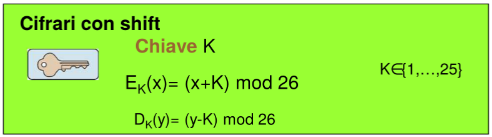
\includegraphics[width=0.8\linewidth]{chapters/chap02/images/shift.png}
\end{figure}

Sono possibili solamente 25 chiavi, è vulnerabile ad un attacco di forza bruta.

\section{Cifrari monoalfabetici}

Viene fatta una sostituzione con un alfabeto cifrante. Sono possibili $26!$ chiavi 
(tutte le possibili combinazioni per l'alfabeto cifrante), ovvero $2^88$.

\subsection{Crittoanalisi}

Potrei pensare di essere al sicuro perché abbiamo un ampio spazio delle chiavi 
(in realtà ad oggi si considera sicuro $2^128$), ma questo schema si può rompere 
con una semplice tecnica di crittoanalisi: \textbf{analisi delle frequenze}.

\section{Cifrario Affine}

Sono un caso particolare dei cifrari a sostituzione monoalfabetica. La sostituzione 
è data da una funzione detta \textit{affine}:


\begin{center}
    $c_i = E(p_i) = (k_1p_i + k_2) mod 26$
\end{center}

$\rightarrow$ la chiave è quindi data da \textbf{due costanti}.

\noindent La \textit{decrittazione} avviene invece secondo la formula:

\begin{center}
    $p_i = D(c_i) = (c_i - k_2) \cdot k_1^{-1}$
\end{center}

\noindent con $k_1^{-1}$ inteso come l'inverso modulo 26 di $k_1$, ovvero quel numero 
$x$ che soddisfa l'equazione:

\begin{center}
    $(k_1 \cdot x) mod 26 = 1$
\end{center}

\noindent Affinché questo sia possibile è necessario che $k_1$ e 26 siano primi tra loro.

\noindent È un altro modo per scrivere la mappatura da un alfabeto in chiaro ad uno 
cifrante; dato che deve essere rispettata la condizione di invertibilità, si ottiene un 
sottoinsieme di tutti i possibili $26!$ alfabeti.

\subsection{Crittoanalisi}

Si riconduce ad un cifrario di sostituzione monoalfabetica, è vulnerabile ad una semplice analisi delle frequenze.

\section{Cifrario di Playfair}

Si ragiona su coppie di caratteri invece che su singoli caratteri: l'idea è che in 
questo modo si ha uno spazio di $26 \cdot 26$, è ancora possibile fare analisi delle frequenze
ma è necessario un testo più ampio.

\begin{figure}[H]
    \centering 
    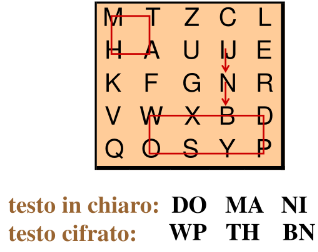
\includegraphics[width=0.8\linewidth]{chapters/chap02/images/playfair.png}
\end{figure}

\noindent Si costruisce un rettangolo $5x5$, mettendo per convenzione nella stessa 
cella le lettere $i$ e $j$; per cifrare viene tracciato un rettangolo tra 
la coppia di lettere, e la cifratura corrisponde ai vertici opposti. 

\noindent Le lettere ripetute vanno separate da una lettera di riempimento (es. $mamma \rightarrow
mamxma$)

\noindent Nel caso di lettere sulla stessa riga o colonna:
\begin{itemize}
    \item stessa riga $\rightarrow$ si sostiuisce con lettere a destra 
    \item stessa colonna $\rightarrow$ si sostituisce con lettere sottostanti
\end{itemize}

\subsection{Crittoanalisi}

È più sicuro rispetto alla cifratura monoalfabetica ($26\cdot26=676$ \textit{digrammi}); è tuttavia 
sempre possibile fare un'analisi delle frequenze dei digrammi.

\section{Cifrario di Hill}

Permette di 
sostituire $m$ lettere in chiaro con $m$ lettere cifrate, usando $m$ equazioni 
lineari. 

\begin{figure}[H]
    \centering 
    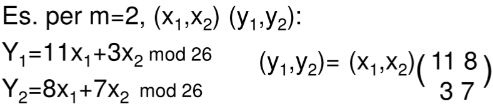
\includegraphics[width=0.8\linewidth]{chapters/chap02/images/hill.png}
\end{figure}

La chiave del cifrario è la matrice, i cui coefficienti vengono scelti in modo arbitrario.

\subsubsection{Esempio}

\begin{figure}[H]
    \centering 
    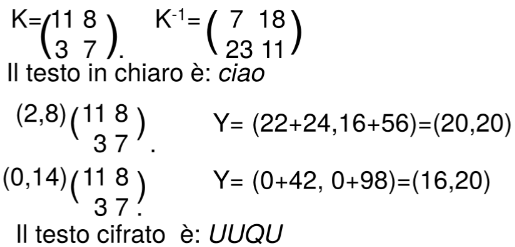
\includegraphics[width=0.8\linewidth]{chapters/chap02/images/hill2.png}
\end{figure}

\noindent Le fasi di cifratura e decifratura, in generale, sono:

\begin{figure}[H]
    \centering 
    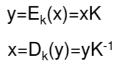
\includegraphics[width=0.8\linewidth]{chapters/chap02/images/hill3.png}
\end{figure}


\section{Cifrario di Vigenère}

\begin{figure}[H]
    \centering
    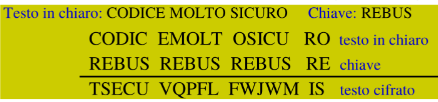
\includegraphics[width=0.8\linewidth]{chapters/chap02/images/vigenere.png}
\end{figure}

\noindent Viene applicato un cifrario di shift per ogni singolo 
caratteri con la parola chiave; si ottiene che si hanno uguali caratteri 
cifrati che corrispondono a lettere in chiaro diverse e viceversa.

\noindent Matematicamente si può rappresentare in questo modo:

\begin{figure}[H]
    \centering
    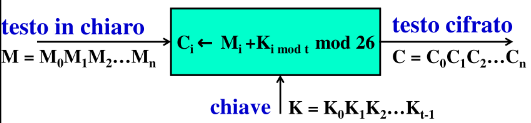
\includegraphics[width=0.8\linewidth]{chapters/chap02/images/vigenere2.png}
\end{figure}

\noindent Sono possibili $26^t$ chiavi, con $t$ lunghezza della chiave.

\section{One-Time-Pad}

È definibile come il cifrario perfetto: viene presa una chiave lunga 
quanto il messaggio, i cui bit sono scelti in modo casuale.

\noindent Il messaggio risulta indecifrabile, perché il crittoanalista non può fare 
alcuna assunzione; il cifrario è \textit{unconditionally secure}, perché a prescindere 
da tempo e risorse computazionali, non è possibile disitnguere quale sia il messaggio 
originale (il massimo che si può ottenere è tutte le possibili frasi di senso compiuto, ma 
senza poter stabilire qual è quella originale).

\begin{figure}[H]
    \centering
    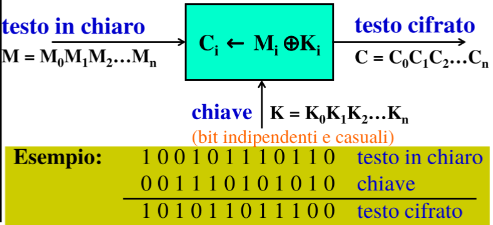
\includegraphics[width=0.8\linewidth]{chapters/chap02/images/otp.png}
\end{figure}

\noindent Il problema è che è necessario avere la chiave lunga quanto il messaggio che ci 
si vuole scambiare.


